\documentclass[10pt]{article}

\usepackage{geometry}
\geometry{margin=2em,top=6em, left=2.5cm, headheight=\paperheight}
\usepackage[export]{adjustbox}
\usepackage{array}
\usepackage{amsmath}
\usepackage{amsfonts}
\usepackage{fancyhdr}
\pagestyle{fancy}
\fancyhf{}
\lhead{Algebra II}
\chead{Function Characteristics - House Prices}
\rhead{Discussion, Page \thepage}
\usepackage{lastpage}
\usepackage{xcolor}
\usepackage{enumitem}
\usepackage{pifont}
\usepackage{graphicx}
\graphicspath{{../img}}
\usepackage{pgfplots}
\pgfplotsset{compat=1.18}
\usepackage{tabularx}

\newcommand{\R}{\mathbb R}
\newcommand{\e}{{\rm e}}
\newcommand{\pobr}[1]{\left\langle#1\right\rangle}
\newcommand{\norm}[1]{\lVert #1 \rVert}
\newcommand{\abs}[1]{\lvert #1 \rvert}

\DeclareMathOperator{\xd}{d\!}
\DeclareMathOperator{\proj}{proj}

\title{}
\date{}

\begin{document}
\noindent
{
Last Name \rule{6em}{.1pt}\hspace{\stretch{1}}First Name \rule{6em}{.1pt}\hspace{\stretch{1}} Date \rule{1.5em}{.1pt} -- \rule{1.5em}{.1pt} -- \rule{1.5em}{.1pt}\hspace{\stretch{1}} Period \rule{2em}{.1pt}\hspace{\stretch{1}} Score \rule{2em}{.1pt}
}
\vspace{1em}

The following chart summarizes the New York house price index in 2021 through 2025.
\begin{figure}[h]
\centering
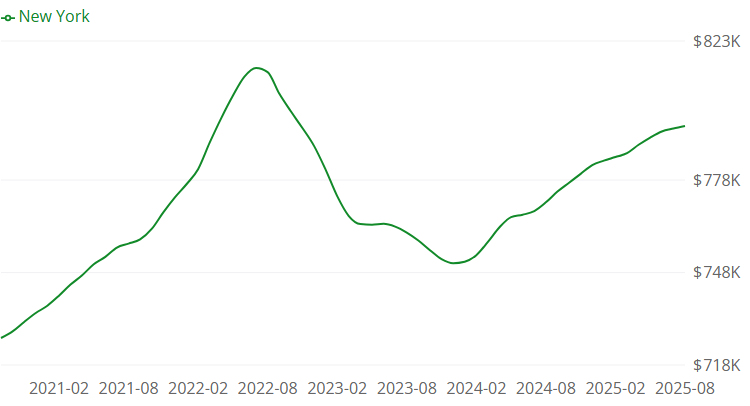
\includegraphics[width=.8\textwidth]{new-york-house-price-2021-2025.png}
\end{figure}
Discuss the following questions.
\begin{enumerate}
\item
If you were planning to buy a house sometime betwee the beginning of 2021 and Auguest 2025, when do you think would be the best time, and why?
\vspace{\stretch{1}}
\item
If you were planning to buy a house sometime between February 2022 and February 2025, when do you think would be the best time, and why?
\vspace{\stretch{1}}
\item 
If you were planning to sell a house sometime betwee the beginning of 2021 and Auguest 2025, when do you think would be the best time, and why?
\vspace{\stretch{1}}
\item
Identify the periods when housing prices were increasing and the net gain in each period.
\vspace{\stretch{1}}
\item
In real life, what are the major difficulties in making investment decisions?
\vspace{\stretch{1}}
\end{enumerate}

\end{document}